%!TEX root = ../../thesis.tex
\renewcommand{\chapterpath}{\allchapterspath/lfui}
\renewcommand{\imgpath}{\chapterpath/img}

\chapter{Learning from Unlabeled Interaction Frames}
\label{chapter:lfui}
\minitoc

Context - Why now: we identified a potential mechanism.

Need - Why the reader: we must now investigate if it can work.

Task - Why me: we developed a new algorithm that formalize the observed constraints depicted before

Object- Why this chapter:  we will start by presenting symbolic experiment where we can observe and maybe prove that the algorithm make sense. We then exemplify on non symbolic data. We then define the terms of the algorithm and the idea of the metric we measure, and the many assumption we do. We then test the algorithm on a pick and place scenario using a 6 dof robot and speech utterances as the modality of interaction.

Findings - What: it works well for feedback and guidance case in 100 or 200 iterations with different classifiers and it is robust to some mistake from the teacher.

Conclusions - So what: So we can envision interacting with system without pre coordination. 

Perspectives - What now: However the question of how the robot should act as been left assigned with random movement or greedy strategies. it has been shown on similar setup but when the signal to meaning is known that learning time can be improve by having an agent seek for more informative signals. Next section present how our robot can plan its action to do better.

%%%%%%%%%%%%%%%%%%%%%%%%%%%%%%%%%%%%%%%%%%%%%%
%%%%%%%%%%%%%%%%%%%%%%%%%%%%%%%%%%%%%%%%%%%%%%
%%%%%%%%%%%%%%%%%%%%%%%%%%%%%%%%%%%%%%%%%%%%%%
%%%%%%%%%%%%%%%%%%%%%%%%%%%%%%%%%%%%%%%%%%%%%%
%%%%%%%%%%%%%%%%%%%%%%%%%%%%%%%%%%%%%%%%%%%%%%
\section{Problem formulation and assumptions}

\subsection{Interaction frame}

\subsection{Learning Algorithm}

%%%%%%%%%%%%%%%%%%%%%%%%%%%%%%%%%%%%%%%%%%%%%%
%%%%%%%%%%%%%%%%%%%%%%%%%%%%%%%%%%%%%%%%%%%%%%
%%%%%%%%%%%%%%%%%%%%%%%%%%%%%%%%%%%%%%%%%%%%%%
%%%%%%%%%%%%%%%%%%%%%%%%%%%%%%%%%%%%%%%%%%%%%%
%%%%%%%%%%%%%%%%%%%%%%%%%%%%%%%%%%%%%%%%%%%%%%
\section{What we exploit}

We assume the system has access to the context in which the task should be executed (e.g. reaching one state among all) and knowns the interaction protocol used by the teacher (e.g. feedback on the agent actions). However the system do not know how to translate signals from the user into their symbolic meaning (e.g. correct/incorrect), neither which particular state it should reach.

Central to our method is a system of hypothesis. By assuming our system has access to the context and the interaction protocol, it can generate hypothesis about the task the human wants it to perform, e.g. reach this or that state. For a particular hypothesis, we can assign hypothetic labels (or meanings) to the human signals knowing their are limited to a fixed set and according to the current state of the world. The machine is ``reasoning'' as follow: \emph{"If the human wants me to solve task $\xi$, then when he said $e$, he meant $l$"}. By creating a set of hypothesis, the system end-up with a set of possible interpretation of the human teaching signals. But as the user have only one objective in mind $\hat{\xi}$, only the correct interpretation will correctly label the signals. 
The key challenge it to find out what it means to correctly label data.

As illustrated in figure \ref{fig:intuition}, our system is looking for the hypothesis from which emerges a coherence between the spacial organization of label in the feature space and their associated labels.

\subsection{Simultaneous Estimation of Task and Signal Model}
\label{sec:Algorithm}
\begin{figure}[!ht]
\centering
    \begin{tabular}{c|c|c}
        \begin{subfigure}[t]{0.29\columnwidth}
            \begin{flushleft}
            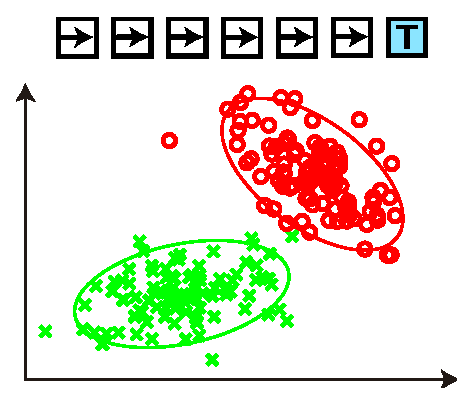
\includegraphics[width=\columnwidth]{\imgpath/GM1}
            \caption{}
            \label{fig:GM1}
            \end{flushleft}
        \end{subfigure}
        &
        \begin{subfigure}[t]{0.29\columnwidth}
            \begin{center}
            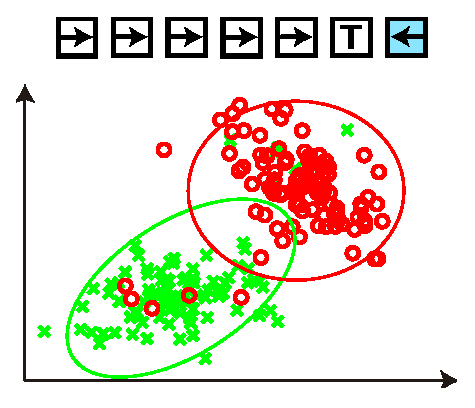
\includegraphics[width=\columnwidth]{\imgpath/GM2}
            \caption{}
            \label{fig:GM2}
            \end{center}
        \end{subfigure}
        &
        \begin{subfigure}[t]{0.29\columnwidth}
            \begin{flushright}
            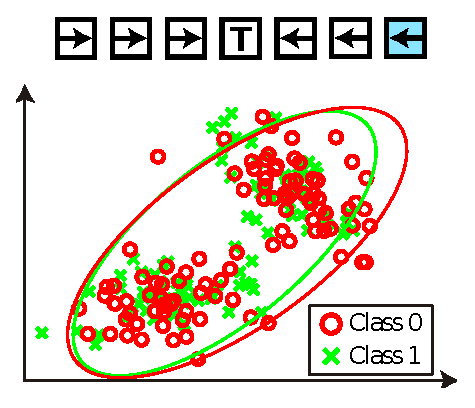
\includegraphics[width=\columnwidth]{\imgpath/GM3}
            \caption{}
            \label{fig:GM3}
            \end{flushright}
        \end{subfigure}
    \end{tabular}
\caption[]{Representation of inferred signal labels for a 1D grid world in function of the hypothesized task. Three task hypotheses are displayed in column from left to right [(a),~(b),~(c)]. On top is a 1D grid world with the hypothetic target state marked with a T letter. Notice that this hypothetic target is different for each of the three hypotheses. The arrows in each cell indicates what action should elicit a positive feedback, i.e.\ the optimal policy with respect to the hypothetic target. The user intended target is shown as the shaded blue state at the right extremity of the 1D world. Note that the system does not have access to this information. The correct hypothesis is the one on the Left [(a)] where the T state is the same as the shaded blue state.
Below the 1D grid world, the signals received from the user are represented in a 2D feature space. They represent the user assessment signals of the past history of device's actions (e.g.\ moving randomly left and right). Our algorithm assigns virtual labels (green for ``correct'' and red for ``wrong'') to those signals with respect to their respective hypothetic target. Notice that the data points are the same for all three hypotheses, only their respective labels differ.
With the virtual labels being assigned, we can compute the corresponding 2D Gaussian distributions estimates for each class (shown as colored ellipses) and each hypothesis. While for the correct hypothesis [(a)] the Gaussian distributions shows a large separability, the overlap increases as the hypothetic target (T) moves away from the real (blue shaded) one [(b), (c)]. This property can be exploited to estimate the correct hypothesis and the model generating the signals.}
\label{fig:GM}
\end{figure}

\subsection{Principle}

The algorithm is  divided into a classification algorithm, estimating one classifier for each hypothesis based on past interaction, and a learning algorithm that uses the results and properties of this classifier to update the belief over hypothesis for current interaction.

Our approach uses the same algorithm if we have label or not. For better explaining the approach, during the explanation we will refer to two phases in the learning process: phase 1 which is learning from scratch a task from unlabelled instruction and phase 2 which is learning a second (or third or) task based on the fact we already inferred a first one. Our algorithm is the same for the two phases but different factor are dominating on one or the other learning phase.

Phase 1 is the main contribution of this work and enable a system to be instructed using signal initially unknown to the it. As stated before, our system will generate hypothesis over the possible task, infer the hypothetic label associated to the signal and check which hypothetic set of signal - label \ldots c nul

Phase 2 seems to be simply learning from known instruction, where a calibration procedure has been performed before. But in our case it differs in one way, we keep generating hypothesis. We keep updating the classifier with the new pair of signal-label from the interaction. Wrong hypothesis will add wrong signal-label to the classifier reducing its quality, so reducing the sharpness of its prediction. The effect will be quite small wrt. the matching process but still helps. In other word we are integrating the fact that the user is not coherent with a hypothesis by integrating new data point in the classifier.

Each hypothesis is believing it is the good one, it is modeling the signal to meaning mapping of the user wrt. the hypothesis objective. Then testing if it can predict the correct label for future interaction. As the user is actually following only one hypothesis, and the signal have some structure in the space, only one hypothesis will be able to predict correctly futture interaction. Our assumption is that the hypothesis which shows more coherence between expected label and predicted label is more likely to be the correct one. 

In phase 1 it is the quality of prediction that differentiate hypothesis. Bad hypothesis will realize that they are not able to predict coherent output, this is mainly measured by the confusion matrix. Realize that if we use a batch method and have an over fitting classifier, no hypothesis will stand out because they will all predict correclty what is going on. With a classifiet that does not overfit, or is just trained on past data, the classifier will still tend to label the data according to the task, because the task is what generates the label (think of symetric hypothesis). But the more we collect data, the more we collect evidence that should make bad hypothesis mix labels, which reduce the quality of the classifier, i.e. it's ability to make correct prediction (different form the probabilitic output of the classifier), which makes the vote of this hypothesis weaker. And here is the trick, the confusion matrix model the noise in the prediction, in our case it can come from noise inherent of the data generation (overlap of distribution) or from teaching mistake (\textbf{teaching mistake with respect to the hypothesis considered}) that both mixes the labels and create non expected prediction from the classifier.

After phase one, we found out which hypothesis was the correct one. We therefore have access to the ``true'' labelling of the data. At this point, we assign the same labels for all hypothesis.

Beginning phase two, all the classifiers are the same, the difference between hypothesis will be on the match between classified signal and expected label. As we interact with the user, some teaching mistake occurs (\textbf{teaching mistake with respect to the hypothesis considered}) that both create non expected prediction from the classifier and decrease the trust I put into my classifier by mixing labels.

So the same process are active in both pahse: non-expected prediction, and decrease of the classifier trust.
In phase one, all hypothesis model there own stuff, there is less non-expected prediction, but the more we interact the less we trust some classifier which mixes labels.
In phase two, all hypothesis start wth the same classifier, there is more non-expected prediciton, and the more we interact the less we trust some classifier which mixes the labels (but here the time to radically change the trust we put in one classifier is long as thay all start with the same data, the more we have similar data the less this plays a role.)

%%%%%%%%%%%%%%%%%%%%%%%%%%%%%%%%%%%%%%%%%%%%%%
%%%%%%%%%%%%%%%%%%%%%%%%%%%%%%%%%%%%%%%%%%%%%%
%%%%%%%%%%%%%%%%%%%%%%%%%%%%%%%%%%%%%%%%%%%%%%
%%%%%%%%%%%%%%%%%%%%%%%%%%%%%%%%%%%%%%%%%%%%%%
%%%%%%%%%%%%%%%%%%%%%%%%%%%%%%%%%%%%%%%%%%%%%%
\section{How do we exploit it}

\subsection{Notations and assumptions}

We consider interaction sessions where a machine is solving a task $\hat{\xi}$ under the supervision of a user who gives feedback (or instructions) to the machine using some specific signal $e$. The machine is ignorant of the task to perform and of the actual meaning of the signals. Its objective is to simultaneously solve the task and learn a model for the user's signals. To achieve this, it has access to a sequence of triplets in the form $\{(s_i, a_i, e_i),\ i = 1,\ldots,M\}$, where $s_i$, $a_i$ and $e_i$ represent, respectively, the state, action and instruction signals at time step $i$. The behavior of the machine is determined by the actions $a\in\mathcal{A}$ and the corresponding transition model $p(s'\mid s,a)$.  We will denote $D_i$ to the history of $(e_i, s_i, a_i)$ up to time $i$.


We make the following assumptions under this general paradigm. First, the system has access to a set of task hypothesis $\xi_1,\ldots,\xi_T$ which includes the task the user wants to solve. We assume instruction signals $e$ have a finite and discrete number of meanings $l \in \{l_1, l_2, \ldots, l_L\}$ which we call labels and this is known by the user and the machine. The simplest example -- the one we will use in the experiments -- is to consider two  possible meanings for the signals: correct or incorrect. We assume that given these labels, it is possible to compute a model that generates or classifies signals $e$ into meanings $l$. The parameters of such a model will be denoted by $\theta$.


%The meaning of  model is unknown at start and is parametrize by $\theta$. Given a label $l$ it outputs the probability that an observed signal $e \in \mathbf{R}^n$ was generated by our model $p(e | l, \theta)$.
 
% the signal-to-meaning mapping. This mapping is done by a classifier parameterize by $\theta$, that is unknown at start. Given a signal $e \in \mathbf{R}^n$ the classifier outputs label probabilities $p(l^{H^\theta} | e, \theta)$.

%We further assume that given a task $\xi$ and a state-action pair $(s, a)$, the machine has access to a model of the user expected labels $p(l^{H} | s, a, \xi)$. We denote as $D_i^\xi$ the history of $(e_i, s_i, a_i, p(l_i^{H} | s_i, a_i, \xi))$ up to time $i$ for task $\xi$. 
%Given $D_i^\xi$, we can optimize the classifier parameters $\theta_i^{\xi}$.


% For each hypothesis, at time $i$, we have several dataset $D_i^{\xi_t}$, which are used to train a classifier parametrize by $\theta_i^{\xi_t}$. Each classifier $\theta_i^{\xi_t}$ represents an interpretation hypothesis of the user given he is trying to instruct the task $\xi_t$.

\subsection{Estimating Tasks Likelihoods}

% \todo{Conceptual terms, no Gaussian classifier, no EEG}

We start by assuming we are provided a calibrated model $\hat{\theta}$ and release this assumption later on.
%
As mentioned in the introduction, knowing $\hat{\theta}$, we can compute the probability of each task $\xi_t$ after observation of a signal $e$ when performing action $a$ in state $s$.

\begin{eqnarray}
p_{\hat{\theta}}(\xi_t|e, s, a ) & \propto & p_{\hat{\theta}}(e |s, a, \xi_t) p(\xi_t)
\label{eq:1}
\end{eqnarray}
where  $p_{\hat{\theta}}(e |s, a, \xi_t)$ takes into account all the probability of each possible meaning $l$ given the target $\xi_t$, the current state $s$ and the action $a$ executed by the machine.
\begin{eqnarray}
p_{\hat{\theta}}(e |s, a,  \xi_t) =  \sum_{k \in {1, \ldots, L}} p_{\hat{\theta}}(e |l = l_k) p(l = l_k| s, a, \xi_t).
\end{eqnarray}

This process can be repeated recursively for several interaction steps $i$, 

\begin{eqnarray}
\L_i^{\xi_t} & = & p(\xi_t|D_i^{\xi_t}, \hat{\theta}) \nonumber \\
& \propto & p_{\hat{\theta}}(e_i |s_i, a_i, \xi_t) p_{ \hat{\theta}}(\xi_t|D_{i-1}^{\xi_t})
\label{eq:filter}
\end{eqnarray}

with $p(\xi_t|D_0^{\xi_t})$ being the prior probability of each task. Also, one can estimate $p(\theta \mid D_i, \xi_{1:i})$, that is, the posterior distribution of the meaning parameters given the task being solved at each point in time. Note the different notation for the task and the meaning parameters. The reason is that $\theta$ is a shared parameter for different tasks, while the task being solved should in principle not affect the meaning of the signals $e$.

%By normalizing the likelihoods of all task, we obtain the probability distribution between tasks. A threshold mechanism could be used to decide when to stop.

We now relax the assumption we are given a model $\hat{\theta}$. The natural extension from the previous models is to compute the posterior distribution over the the task and the model, $p(\xi_t, \theta^{\xi_t} |e, s, a)$. However, the resulting distribution does not have a close form solution even when linear Gaussian likelihoods are used due to the combination of mixtures for each possible task. Another alternative is to compute the $\theta$ and $\xi$ that maximize the data likelihood. This is prone to fail in certain scenarios due to two reasons. First, it is common that different tasks share many labels (e.g. the policies to reach neighboring cells on a grid world are almost identical and, therefore, share most of the labels $l$) and results on large uncertainties in the task space that require multiple actions to be disambiguated. Second, if the signals are not well separated the meaning parameters $\theta$ of different tasks will not differ much.  

For instance, under Gaussian assumptions for $p_{\theta}(e |l = l_k)$ and deterministic task labels $p(l = l_k| s, a, \xi_t)$, it is possible to integrate out  $\theta$ to compute the marginal likelihood $p(D_i\mid \xi)$. The resulting likelihood depends only on the traces of each $p_{\theta}(e |l = l_k)$. Empirical results with synthetic and EEG data for a reaching task on a grid revealed that, when the distributions over $e$ overlap, the traces were not enough to recover the most likely task and the corresponding meaning parameters. 

To cope with these problems, we define the following pseudo-likelihood function 

\begin{eqnarray}\label{eq:pseudo1}
\lefteqn{P(D_n | \xi, \theta) \approx \prod_{i=1}^N p(e_i | \xi, \theta_{-i},s_i,a_i)}  \\ \label{eq:pseudo2}
&=& \prod_{i=0}^N \sum_{l_c}\sum_l  p(e_i | \theta_{-i}, l_c)  p(l_c | \theta_{-i},l) p(l|\xi,s_i,a_i), 
%p(\xi_t, \theta^{\xi_t} |e, s, a) & \propto & p(e | s, a, \xi_t, \theta^{\xi_t}) p(\xi_t, \theta^{\xi_t}).
\label{eq:}
\end{eqnarray}

where $l$ represents the the meaning assigned by task $\xi$, action $a_i$ and state $s_i$ and $l_c$ is the label according to the meaning model $\theta_{-i}$ for a given label $l$.

The pseudo-likelihood is built using a leave-one-out cross-validation strategy to evaluate the likelihood $p(e_i | \xi, \theta_{-i},s_i,a_i)$ of each signal based on the meaning parameters $\theta_{-i}$ learned for each task using all the other available signals. The rationale behind it is that for the correct task, the labels and signals will be more coherent than for other tasks resulting in higher likelihoods. If we interpret $p(e_i | \xi, \theta_{-i},s_i,a_i)$ as a classifier, its predicted labels match the ones provided by the task for different state-actions pairs. Note that wrong tasks assign wrong labels $l$ to the signals $e$ and, therefore, the learned models will have larger overlaps. 

Each term of the pseudo-likelihood is computed from three terms. $p(l|\xi,s_i,a_i)$ represents the probability distributions of the meanings according to the task, the executed action and the current state.   $p(l_c | \theta_{-i},l)$ encodes which label will be actually recovered by $\theta_{-i}$. Intuitively, it models the quality of the model $\theta_{-i}$. $p(e_i | \theta_{-i}, l_c)$ is the likelihood of the signal given the meaning. 
%
The pseudo-likelihood is maximized in two steps. First, the maximum a posteriori estimate for each $\theta_{-i}$ of each task  is computed. Then, the term $p(l_c | \theta_{-i},l)$ is approximated by the corresponding confusion matrix of a classifier based on $\theta_{-i}$. Finally, the best task $\xi$ is the one that maximizes the pseudo-likelihood in Eq. \ref{eq:pseudo1}.

\subsection{Decision and Task Change}

The machine is simultaneously solving a task and learning the meanings associated to the signals. However, it is possible to solve the task before the meanings are perfectly modeled or vice-versa. Therefore, in practical terms it is necessary to be able to switch to the next task once it has been solved and to continue updating the meaning. 
%
We define $W^{\xi_t}$ the minimum of pairwise normalized likelihood between hypothesis $\xi_t$ and each other hypothesis: 

\begin{eqnarray}
W^{\xi_t} = \argmin_{x~\in~{1, \ldots, T} \smallsetminus \{t\}} \frac{P(D_n | \xi_t, \theta)}{P(D_n | \xi_t, \theta) + P(D_n | \xi_x, \theta)}.
\label{eq:weight}
\end{eqnarray}

When it exists a $t$ such that $W(\xi_t)$ exceeds a threshold $\beta \in ]0.5,1]$ we consider task $\xi_t$ is the one taught by the user.

After identifying a task, we can infer the true labels of the past data and assign such labels for all hypothesis. The user starts teaching a new task using the same kind of signals. By using the same algorithm we can start learning this new task faster as all hypothesis share a common set of signal-label pairs. The meaning model is still updated step after step until next task is identified and labels reassigned.

\subsection{stuff}


This section formalizes the problem of executing a task when the mapping between raw EEG signals to a discrete label among a set of pre-defined labels is unknown. The main idea is depicted in Figure~\ref{fig:GM} for a toy 1D example. The user wants the device to reach the right-most state. For each device's action, he provides a feedback signal which encode whether the action executed is ``correct'' or ``wrong'' according to the intended target. Such signals are generated from an underlying model which maps a binary label (``correct'' or ``wrong'') to a continuous signal. However, neither the user's desired target nor the labels associated to the user's feedback signals are known.

Considering that we can define a finite set of task hypotheses (e.g. reaching one of a finite number of states), we can infer the labels that should be provided by the user with respect to each hypothesis. Then, given a particular interaction history, it is possible to compute a different signal decoder for each task hypothesis. The key point is that only the correct hypothesis will assign the correct labels to all feedback signals (Figure~\ref{fig:GM1}), while the other hypotheses will gradually mix both classes as the hypothetic target gradually differs more from the correct one (Figure~\ref{fig:GM2}~and~\ref{fig:GM3}). Therefore, the hypothesis which provides the decoder with best accuracy and compactness can be selected as the most probable one. In the remainder of this section we show how this property can be exploited to estimate the target and the model generating the feedback signals.

Formally, we represent the problem as a discrete or continuous set of states $s \in S$,  a finite set of possible actions $a \in A$, and a set of possible tasks, or targets, for which the system is able to plan the best sequence of actions. In the 1D example in Figure~\ref{fig:GM}, the state space is composed of seven discrete states, and the agent can perform unitary directional actions, i.e. move one cell left or right. During an interactive learning session, the agent will proactively perform actions which will in turn be evaluated as ``correct'' or ``wrong'' by the user with respect to the desired target state on the grid. In our case the feedback signals are error-related potentials measured in the brain activity of the subject.

Let $e_i\in \mathbf{R}^n$ denote the feature vector of the EEG measurements obtained at iteration $i$ after the device performed action $a_i$ in state $s_i$. The label $z_i\in\{c,w\}$ of each feedback signal belongs to one of two classes (``correct'' or ``wrong'').
%
Following \cite{blankertz2010single} (\cite{blankertz2010single}), we will model the EEG signals using independent multivariate normal distributions for each class ($\mathcal{N}(\mu_c, \Sigma_c)$ and $\mathcal{N}(\mu_w, \Sigma_w)$). We will denote by $\theta$ this set of parameters $\{\mu_c, \Sigma_c,\mu_w, \Sigma_w\}$.

We assume the system has access to a set of task hypotheses $\xi_1,\ldots,\xi_T$ which includes the task the user wants to solve. We do not make any particular assumption on how the task is represented but we assume that for each particular task $\xi$ we are able to compute a policy $\pi_\xi$ which represents the probability of choosing a given action $a$ in state $s$, $\pi_{\xi}(s,a) = p(a|s,\xi)$. As mentioned above, these are the policies that, conditioned on the task, provide labels to the feedback signals of a state-action pair (e.g. in a reaching task, progressing towards the goal will generate ``correct'' feedback while moving apart from it will generate ``wrong''feedback).

The method aims to infer which task $\hat{\xi}$ the user wants to solve based on the user's feedback signals extracted from EEG measurements collected while the agent executes some actions. Following the analysis of Figure~\ref{fig:GM}, a sensible option to estimate the task is to measure the coherence of the signal model for each possible task using the virtual labels provided by the target policy. In other words, the best $(\xi,\theta)$ pair provides the lowest predictive error on the observed signals $p(e|s,a,\xi,\theta)$, which themselves were collected in the recent history of interaction. One possible way of solving this problem is to maximize the expected classification rate:
%
\begin{eqnarray}
\hat{\xi},\hat{\theta}&=& \arg\max_{\xi,\theta} E_e\left[ \delta(z(s,a,\xi), z(e,\theta)) \right]
\end{eqnarray}
%
where $\delta()$ is an indicator function, $z(s,a,\xi)$ is the label (correct or wrong) corresponding to the execution of action $a$ in state $s$ under task $\xi$ and $z(e,\theta)$ is the label provided by classifying the EEG signal $e$ under the Gaussian classifier parameterized by $\theta$. The expected classification rate ($Ecr$) can be explicitly written dependent on the task and decoder model:
%
\begin{eqnarray}
\lefteqn{Ecr\left( \delta(z(s,a,\xi), z(e,\theta)) \right) =}\nonumber\\
 &=& \sum_{k \in \{c,w\}} p(z=k|s,a,\xi) p(z=k|e,\theta)
\label{eq:ecr} 
\end{eqnarray}
%
where $p(z=k|s,a,\xi)$ represents the probability of the user assigning label $k$ when assessing action $a$ in state $s$ according to task $\xi$. We add a noise term to cope with those situations where the user assessment may be wrong. The model for probability of correct assessment is then:
%
\begin{equation}
    p(z=c|s,a,\xi) = \begin{cases}
                           1-\alpha           & if~a = \arg\max_{a} \pi_{\xi}(s,a)\\
                           \alpha             & \text{otherwise}\\
                       \end{cases}
\end{equation}
%
with $\alpha$ modeling the assessment error rate of the user, which was set to $0.1$ for our experiments.

Finally, the term $p(z=k|e,\theta)$ is just the probability that the signal $e$ belong to class $k$ under the Gaussian model provided by $\theta$ and is given by:
%
\begin{eqnarray}
    p(z=k|e,\theta) &=& 
                \frac{p(e|z=k, \theta)p(z = k)}{\sum_{l \in \{c,w\}}{p(e|z=l,\theta)p(z=l)}}\nonumber\\
                 &=& \frac{\mathcal{N}(e|\mu_k, \Sigma_k)p(z = k)}{\sum_{l \in \{c,w\}}{\mathcal{N}(e|\mu_l, \Sigma_l)p(z=l)}}
    \label{eq:dev}
\end{eqnarray}
%
As we do not have a priori knowledge on the user intended meaning, we assume that it is equiprobable $p(z = c) = p(z = w)$. We will factorize the optimization process using the fact that given a task $\xi$, the estimation of $\theta$ under the Gaussian model is straightforward. It basically requires to compute the maximum-likelihood estimate $\theta^{ML}_{\xi}$ using the labels associated to target $\xi$. We could also consider a prior distribution on the parameters and update it with new observations. Using the labels of target $\xi$, the estimation of $\theta$ under the Gaussian model described above simply returns to the computation of the posterior mean $\mu_z$ and covariance $\Sigma_z$ for each class $z \in \{c, w\}$. In order to avoid numerical problems when estimating the covariance for a low number of examples, a regularization term was applied to penalize very large and very small eigenvalues \cite{friedman1989regularized}:
%
\begin{eqnarray}
\Sigma_z = (1-\lambda)\Sigma_z + \lambda \frac{trace(\Sigma_z)}{n} \textbf{I}_n
\end{eqnarray}
%
with n the feature dimension, $\textbf{I}_n$ the identity matrix of size $n$, and $\lambda$ the regularization term which was set to $0.5$ for our experiments. An automatic adaptation of the regularization could also be considered \cite{ledoit2004well}.

Using equation~\ref{eq:ecr} to estimate the expected classification rate is difficult because we ideally want to estimate it on future, never observed, data. A possible solution is to use cross-validation or bootstrapping methods using the available data. However, for small amounts of data, these methods result in estimates with high variance \cite{bengio2004no} and computational cost.

Alternatively, we propose to use another approximation of the expected classification rate, the Bhattacharyya coefficient. This coefficient has been related to the classification error of Gaussian models \cite{Kailath67} and is inversely proportional to the classification rate. Although there is no analytical relation between the coefficient and the classification rate, it is possible to derive bounds and good empirical approximations \cite{lee2000bayes}.
%
The Bhattacharyya coefficient $\rho \in [0,1]$ between the Gaussian distributions associated to label ``correct'' ($\mathcal{N}(\mu_c, \Sigma_c)$) and ``wrong'' ($\mathcal{N}(\mu_w, \Sigma_w)$) is:
%
\begin{eqnarray}
\rho = e^{-D_B(\theta)}
\end{eqnarray}
%
where $D_B$ is the Bhattacharyya distance:
$D_B(\theta)=$\\$\frac{1}{8}(\mu_c-\mu_w)^T(\frac{\Sigma_c+\Sigma_w}{2})^{-1}(\mu_c-\mu_w)+\frac{1}{2}ln\left(\frac{det(\frac{\Sigma_c+\Sigma_w}{2})}{\sqrt{det\Sigma_c det\Sigma_w}}\right)$. 

Finally, we approximate the expected classification rate as: 
\begin{eqnarray}
Ecr \propto 1 - \rho
\end{eqnarray}


\subsection{Confidence on Target Estimation}

Now that we have an estimation of the expected classification rate, we need to take a decision with respect to which task is the one intended by the user. To do so we should compare the expected classification rate of every task hypothesis $\xi_t$ with $t \in \{1, \ldots, T\}$. The hypothesis whose associated model has the highest expected classification rate, i.e.\ the lowest value of $\rho$, is expected to be the one intended by the user, however it is meaningless to define an absolute threshold on the value of the expected classification rate itself. Indeed, different people generate different signals which result in classifiers of different qualities. To bypass this problem we rely on a voting system where we attribute each hypothesis $\xi_t$ a weight that is updated at every iteration.

We rely on a pseudo-likelihood metric that for each hypothesis $\xi_t$ accumulate expected classification rate over time:
%
\begin{eqnarray}
\L(\xi_t) = \prod_{i = 1}^{N} 1 - \rho_i^{\xi_t}
\end{eqnarray}
%
with N the current number of iteration and $\rho_i^{\xi_t}$ the Bhattacharyya coefficient associated to task $\xi_t$ using all data up to time $i$. By normalizing the pseudo-likelihood values between every hypothesis, we obtain what can be viewed as the probability of each target:
%
\begin{eqnarray}
p(\xi_t) = \frac{\L(\xi_t)}{\sum_{u \in \{1, \ldots, T\}} \L(\xi_u)}
\end{eqnarray}
%
Once a target reaches a probability threshold $\beta$ we consider it as being the correct one, i.e.\ the one intended by the user. We used $\beta = 0.99$.

\subsection{Estimation of further Tasks and Online Re-Estimation of Signal Model}
\label{sec:AlgReUse}

Once we have identified a first task, the user can change his desired target and our system has to identify the new target. However, the model of the feedback signals does not change and does not have to be re-learned from scratch. Indeed, once the system has correctly identified a task, it is possible to reuse acquired data by assigning to all the previously collected signals the labels associated to the previously estimated task. 

The use of the Bhattacharyya coefficient provides a simple and efficient way to estimate a first target from scratch (when the number of examples is small) but does not allow a fast adaptation to new targets as the majority of collected signals now belong to the previous task. To avoid this problem we compute a classifier (e.g. a Gaussian Bayes classifier), and use it similarly to calibrated approaches in BCI. For this we factorize the joint distribution:
%
\begin{eqnarray}
p(\xi_t, \theta \mid D^{\xi_t}_i) & \propto & p(\xi_t \mid D^{\xi_t}_i)p(\theta \mid \xi_t, D^{\xi_t}_i)
\end{eqnarray}
%
where $D^{\xi_t}_i$ contains all the quadruplet $(e_i,s_i,a_i,z_i)$ up to time $i$, with the associated labels $z_i$ assigned with respect to task $\xi_t$. The factorization makes explicit that given the task $\xi_t$, the distribution $p(\theta \mid \xi_t, D^{\xi_t}_i)$ can be easily evaluated using the labels of each target. We approximate this posterior using the maximum likelihood point estimate $\theta^{ML}_{\xi_t}$ per target. For the term $p(\xi_t \mid D^{\xi_t}_i)$, we use a recursive Bayes filter:
%
\begin{eqnarray}
p(\xi_t \mid D^{\xi_t}_i) &\propto & p(e_i \mid \xi_t, (s,a)_i,D^{\xi_t}_{i-1})p(\xi \mid D^{\xi_t}_{i-1}) \nonumber\\
& \approx & p(e_i\mid \theta^{ML}_{\xi_t})p(\xi_t \mid D_{i-1}).
\label{eq:taskprob}
\end{eqnarray}
%
Notice that we are keeping a different symbol model  $\theta^{ML}_{\xi_t}$  for each possible target $\xi_t$, the maximum likelihood estimation needs to be done in relation to a dataset $D^{\xi_t}_{i-1}$ which include the expected labels of target $\xi_t$ up to time $i-1$. 

We use the same threshold mechanism as described in previous subsection to decide whether or not a task can be considered the correct one. Whenever a task is identified, its labels are transferred to the quadruplets $D^{\xi_t}_{i}$ of all the other tasks to correct the prior for the next step with the right labels. This scheme performs a long term adaptation of $\theta$ to accommodate slight variations of EEG such as non-stationarities or variations induced by the task. 

However, as tasks are identified, the prior becomes more informative and the adaptation may have problems to cope with drastic changes such as strongly modifying the signals. To handle this problem, we chose to limit the size of the prior through the use of a sliding window on past iterations which allows to estimate a moving average of parameters $\theta$. In practice, we limited $D^{\xi_t}_{i}$ to the last $250$ elements.

\subsection{Using known signals}

%%%%%%%%%%%%%%%%%%%%%%%%%%%%%%%%%%%%%%%%%%%%%%
%%%%%%%%%%%%%%%%%%%%%%%%%%%%%%%%%%%%%%%%%%%%%%
%%%%%%%%%%%%%%%%%%%%%%%%%%%%%%%%%%%%%%%%%%%%%%
%%%%%%%%%%%%%%%%%%%%%%%%%%%%%%%%%%%%%%%%%%%%%%
%%%%%%%%%%%%%%%%%%%%%%%%%%%%%%%%%%%%%%%%%%%%%%
\section{Method}

In this section we present results from our algorithm both in simulation and with a real robotic system where we test different aspects: a) learning the associated meaning of instruction words while learning a new task, b) extend it for the case of guidance words, c) combine learning from unknown signals with pre-defined signals of known meanings, d) reuse learnt signals-to-meaning association for the learning of a new task.

We construct a small size pick-and-place task with a real robot. This robot is going to be programmed using a natural speech interface whose words have an unknown meaning and are \textbf{not} transformed into symbols via a voice recognizer. The robot has a prior knowledge about the distribution of possible tasks.

The interaction between the robot and the human is a turn taking social behavior, where the robot performs an action and waits for a feedback, or guidance, instruction to continue. This allows to synchronize a speech wave with its corresponding pair of state and action. The experimental protocol is summarized in figure \ref{fig:lfui:bloc}.

\begin{figure}[!htbp]
  \centering
  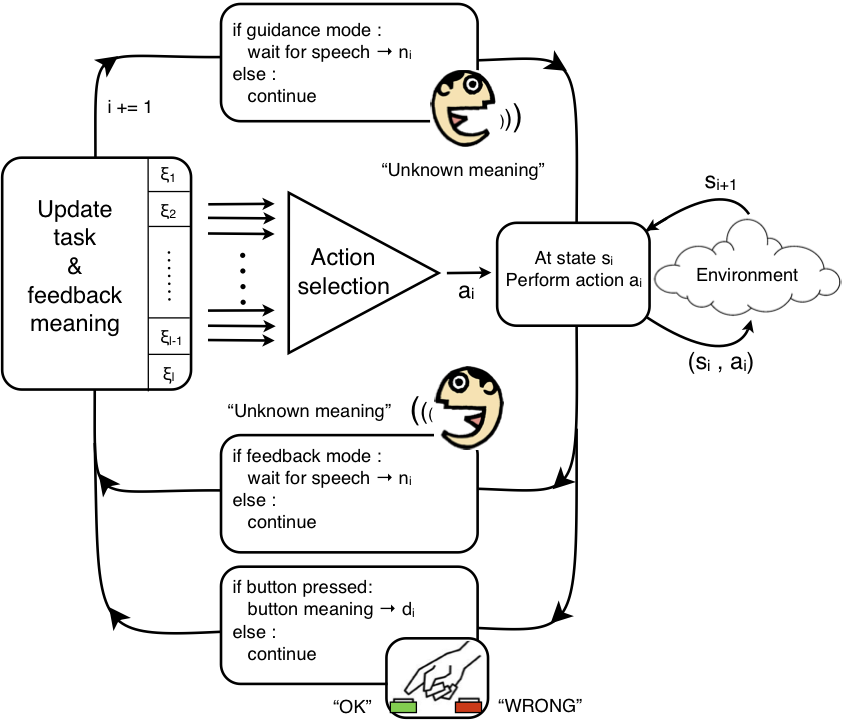
\includegraphics[width=\columnwidth]{\imgpath/bloc.png}
  \caption{Experimental protocol showing the interaction between the teacher and the learning agent. The agent has to learn a task and the meaning of the instructions signals provided by the user, here recorded speech. The teacher can use guidance or feedback signals but has also access to buttons of known meaning for the robot.}
  \label{fig:lfui:bloc}    
\end{figure}

\subsection{Robotic System}

We consider a six d.o.f. robotic arm and gripper that is able to grasp, transport and release cubes in four positions. We used a total of three cubes that can form towers of at most two cubes.  The robot has 4 actions available: \textit{rotate left}, \textit{rotate right}, \textit{grasp cube} and \textit{release cube}. The state space is discrete and defined as the location of each object, including being on top of another or in the robot's gripper. For a set of 3 objects we have 624 different states. Figure~\ref{fig:lfui:setup} shows the robot grasping the orange cube. 

\begin{figure}[!htbp]
  \centering
  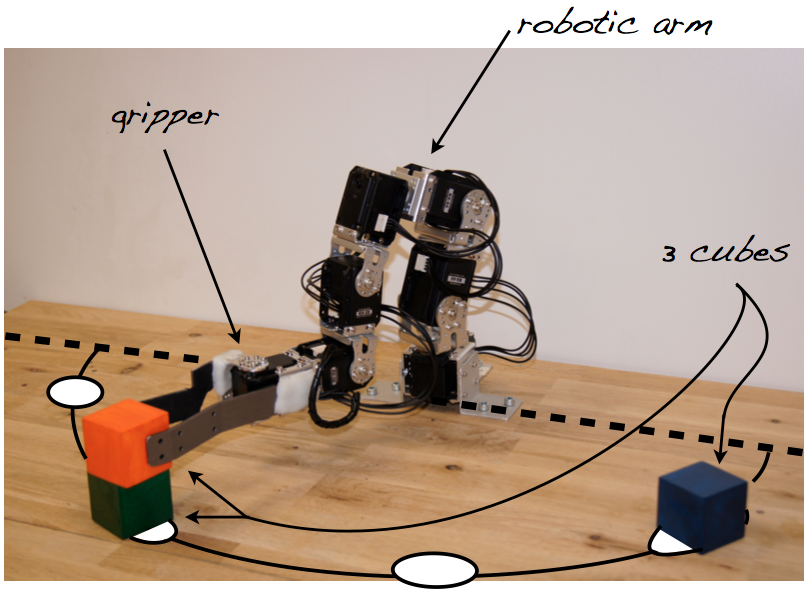
\includegraphics[width=\columnwidth]{\imgpath/setup.png}
  \caption{Robotic System. A six d.o.f robotic arm and gripper learning to performing a pick-and-place task with three cubes.}
  \label{fig:lfui:setup}
\end{figure}

\subsection{Task Representation}

We assume that for a particular task $\xi$ we are able to compute a policy $\pi$ representing the optimal actions to perform in every state. One possibility is to use \textit{Markov Decision Processes} (MDP) to represent the problem \cite{sutton1998reinforcement}. From a given task $\xi$ represented as a reward function we can compute the corresponding policy using, for instance, Value Iteration \cite{sutton1998reinforcement}. In any case, our algorithm does not make any assumption about how tasks are represented.

For this particular representation we assume that the reward function is sparse and so we can generate possible tasks by sampling sparse reward functions consisting of a unitary reward in one state and no reward in all the other. In other words the task is to reach one, yet unknown, of the 624 states of the MDP.

Under this formalism the action selection at runtime can be done in different ways. As different sampling methods can lead to different learning behaviors we will compare two different methods: random and  $\epsilon$-greedy. When following random action selection the robot does not use its current knowledge of the task and randomly select actions. Whereas with $\epsilon$-greedy method the robot performs actions according to the current belief of what the task is, i.e. following the policy corresponding to the most likely task hypothesis. The corresponding optimal action is chosen with $1-\epsilon$ probability, otherwise, a random one is selected. In our experiment we show only results with $\epsilon =  0.1$. 

\subsection{Feedback and Guidance Model}

From a given task $\xi$, we can compute the corresponding policy $\pi^{\xi}$. This policy allows to interpret the teaching signals with respect to the interaction protocol defined. 

In this work, we will consider the user is providing either feedback or guidance on the agent's actions. For the feedback case, we define $p(z |s, a, \xi)$ as:

\begin{equation*}
    p(z = \emph{correct} |s,a,\xi) = 
    \begin{cases}
    1-\alpha               & if~a = \argmax_a \pi^{\xi}(s,a)\\
        \alpha             & \text{otherwise}\\
   \end{cases}
\end{equation*}
with $\alpha$ modeling the expected error rate of the user and $p(z = wrong |s,a,\xi) = 1 - p(z = correct |s,a,\xi)$.

For the guidance case, we define $p(z |s, \xi)$ for each action as (the action being the intented meaning of the user):

\begin{equation*}
    p(z = a |s,\xi) = 
    \begin{cases}
        1-\alpha              & if~a = \argmax_a \pi^{\xi}(s,a)\\
        \frac{\alpha}{3}             & \text{otherwise}\\
   \end{cases}
\end{equation*}
with $\alpha$ modeling the expected error rate. As the agent can perform 4 different actions, we used the constant $\frac{\alpha}{3}$ in order to conserve the property $\sum_a p(z = a |s,\xi) = 1$.

For all experiments $\alpha$ was set to $0.1$.

\subsection{Speech Processing}

As mentioned before, we consider speech as the modality for interacting with the robot. After each action we record the teaching word pronounced by the user. This data is mapped into a $20$ dimensional feature space using the methodology described next.  

A classical method for representing sounds is the \textit{Mel-Frequency Cepstral Coefficients} (MFCC) \cite{zheng2001comparison}. It represents a sound as a time sequence of MFCC vectors of dimension $12$. Comparing sounds is done via \textit{Dynamic Time Warping} (DTW) between two sequences of feature vectors \cite{sakoe1978dynamic}. This distance is a measure of similarity that takes into account possible insertions and deletions in the feature sequence and is adapted for comparing sounds of different lengths. Each recorded vocal signal is represented as its DTW distance to a base of 20 pre-defined spoken words which are \textbf{not} part of words used by the teacher.

By empirical tests on recorded speech samples, we estimate that a number of 20 bases words were sufficient and yet a relatively high number of dimensions to deal with a variety of people and speech. This base of 20 words has been randomly selected and is composed of the words:\emph{ \footnotesize{Error, Acquisition, Difficulties, Semantic, Track, Computer, Explored, Distribution, Century, Reinforcement, Almost, Language, Alone, Kinds, Humans, Axons, Primitives, Vision, Nature, Building}}.


\subsection{Classification System for the Instruction Model}

As explained in section, any standard machine learning classifier can be used for approximating the instruction model. If such classifier is not able to use probabilistic labels then the maximization step of the EM algorithm is approximated in Eq. \ref{eq:F} with a hard thresholds for $z_i^{\xi}$. We then have to rely on the generalization performances of the classifier. Indeed, if the classification algorithm is overfitting the data then no differences can be found between the different hypotheses. The only required characteristic is the ability to output a confidence on the class prediction, i.e. a probability for $n_i$ of being associated to each meaning.

In this study we decided to compare three classifiers for the instruction learning, i.e. modeling $p(n|z,\theta)$:
\begin{itemize}
\item Gaussian Bayesian Classifier: Computing the weighted mean $\mu$ and covariance matrix $\Sigma$, the usual equations for Gaussian mixture hold.
\item Support Vector Machine (SVM): Using a RBF kernel with $\sigma = 1000$ and $C = 0.1$. The parameter values have been estimated via a swap of parameters and by estimating performances via a cross validation procedure on the dataset. For SVM probabilistic prediction refer to \cite{platt1999probabilistic}.
\item Linear Logistic Regression: The predictive output value ([0,1]) is used as a measure of confidence.
\end{itemize}

%%%%%%%%%%%%%%%%%%%%%%%%%%%%%%%%%%%%%%%%%%%%%%
%%%%%%%%%%%%%%%%%%%%%%%%%%%%%%%%%%%%%%%%%%%%%%
%%%%%%%%%%%%%%%%%%%%%%%%%%%%%%%%%%%%%%%%%%%%%%
%%%%%%%%%%%%%%%%%%%%%%%%%%%%%%%%%%%%%%%%%%%%%%
%%%%%%%%%%%%%%%%%%%%%%%%%%%%%%%%%%%%%%%%%%%%%%
\section{Results}

Experiments presented in this section follow the protocol described in figure~\ref{fig:lfui:bloc}, where each turn the agent performs one action and waits for the teaching signals from the teacher. We first present a set of simulated experiments using the same MDP as for the real world experiment. We start by assuming that the teacher provides feedback instructions without any mistakes, therefore only the variability in the signals remains. We compare first the different classifiers, and then the performances of $\epsilon$-greedy versus random action selection methods both for feedback and guidance modes. Later, we present an analysis of robustness to teacher mistakes. The last simulated experiment studies the case where the teacher has also access to buttons of known meaning. Finally, we show the result using a real robot where we study how signals knowledge learned in a first run can be used in a second one to learn more efficiently.

In order to be able to compute statistically significant results for the learning algorithm, we created a database of speech signals that can be used in simulated experiments. All results report averages of 20 executions of the algorithm with different start and goal states. By normalizing the cumulative likelihood estimates $q_1,\ldots,q_T$ (see Algorithm~\ref{alg:interlearn}) to 1, we obtain the probability that each particular task hypothesis represent the task to learn.

\subsection{Learning feedback signals}

In this experiment we assume that the robot does not know the words being spoken by the teacher and he does not know the task either. The teacher is providing instruction whose meaning is either \texttt{correct} or \texttt{wrong}. The robot will, simultaneously, learn the task and map the words that is recorded into a binary feedback signal.

The results comparing the different classification methods are shown in Figure~\ref{fig:FeedbackOneWord}. Action selection is done $\epsilon$-greedy. Note that after 200 iterations all three methods have identified the correct task, i.e. the normalized goal likelihood value is greater than 0.5, meaning that the sum of all the others is inferior to 0.5. Logistic regression provides the worse results in terms of convergence rate and variance.

\begin{figure}[!htbp]
  \centering
  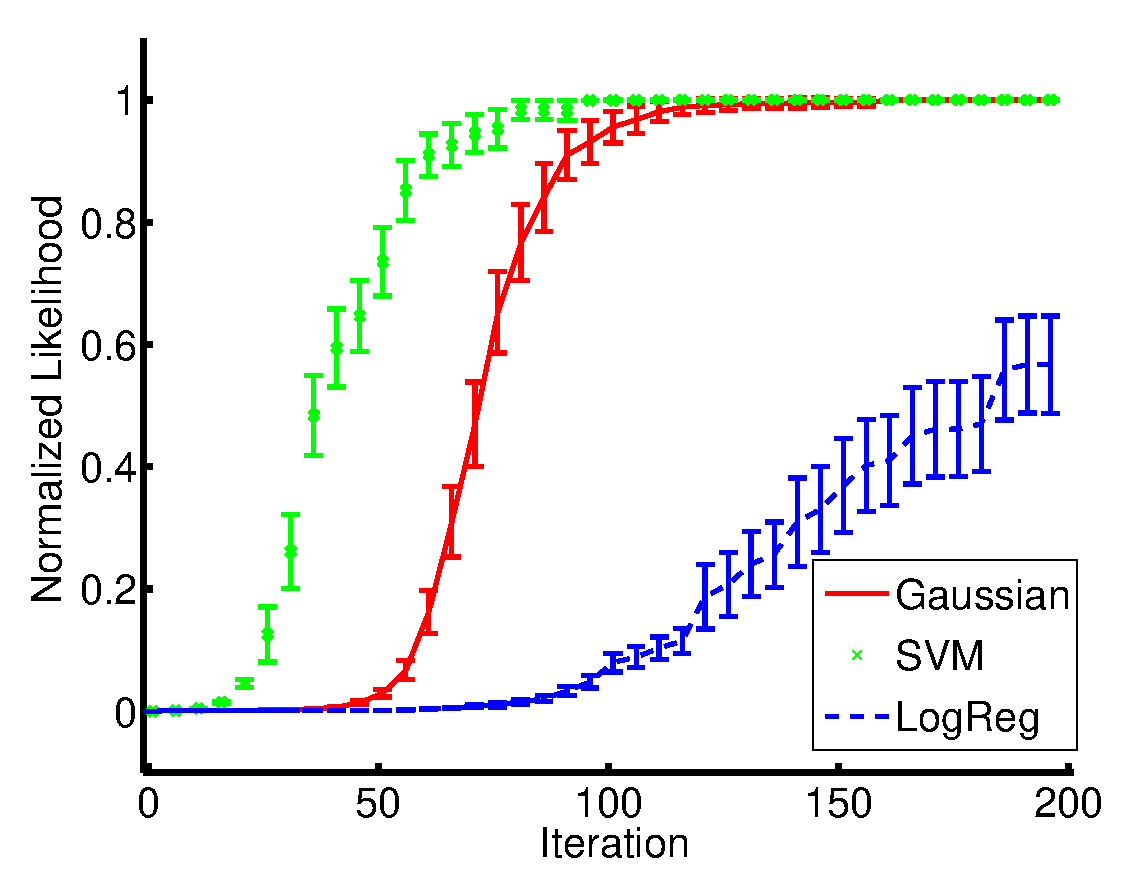
\includegraphics[width=\columnwidth]{\imgpath/classifiers}
  \caption{Taught hypothesis normalized likelihood evolution (mean + standard error) thought iteration using different kinds of classifiers. The teacher is providing feedback using one word per meaning and the agent is performing action according to $\epsilon$-greedy strategy.}
  \label{fig:FeedbackOneWord}
\end{figure}

The user is not restricted to the use of one word per meaning, Table~\ref{tab:1} compares the goal normalized likelihood value after 100 iterations for feedback signals composed of one, three and six spoken words per meaning. SVM has better performance when using one word per meaning but the Gaussian classifier has overall better results with less variance, see Table~\ref{tab:1}. 

\begin{table}[htbp]
\centering
\begin{tabular}{|l|c|c|c|}
\hline
&\textbf{One word}&\textbf{Three words}&\textbf{Six words}\\\hline
\textbf{Gaussian}&1.0 (0.1)&1.0 (0.1)&0.7 (0.1)\\\hline
\textbf{SVM}&1.0 (0.0)&0.5 (0.4)&0.3 (0.4)\\\hline
\textbf{LogReg}&0.1 (0.1)&0.2 (0.3)&0.2 (0.3)\\\hline
\end{tabular}
\caption{Taught hypothesis normalized likelihood values after 100 iterations (mean and standard deviation). Comparison for different classifiers and number of words per meaning. The Gaussian classifier has overall better performances.}
\label{tab:1}
\end{table}

\begin{table}[!t]
\caption{Taught hypothesis normalized likelihood values after 100 iterations (mean and standard deviation). Comparison for different classifiers and number of words per meaning. The Gaussian classifier has overall better performances.}
\vspace{1em}
\centering
\begin{tabular}{|l|c|c|c|}
\hline
&\textbf{One word}&\textbf{Three words}&\textbf{Six words}\\\hline
\textbf{Gaussian}&1.0 (0.1)&1.0 (0.1)&0.7 (0.1)\\\hline
\textbf{SVM}&1.0 (0.0)&0.5 (0.4)&0.3 (0.4)\\\hline
\textbf{LogReg}&0.1 (0.1)&0.2 (0.3)&0.2 (0.3)\\\hline
\end{tabular}
\end{table}

Interestingly the Gaussian classifier learns better after 100 iterations than the other classifiers with many words per meaning. This counter intuitive result can be explain by the high dimensionality of the space where even one Gaussian can differentiate several group of clusters. Linear logistic regression have lower performance presumably due to the linear decision boundary. For the SVM classifier, which is kernalized, as only 100 data points are distributed between each cluster, the more the number of cluster increase the less data point per cluster. The iterative fitting process of the SVM is therefore more likely to consider some data as noise, omitting some clusters. For the following experiments, we will only consider the Gaussian classifier, first because it has overall better performance but also because it is the faster to train and thus is the only one usable for real world and real time experiments. Indeed, in this setup, at each iteration the agent has to train 624 classifiers.

\begin{figure}[!htbp]
  \centering
  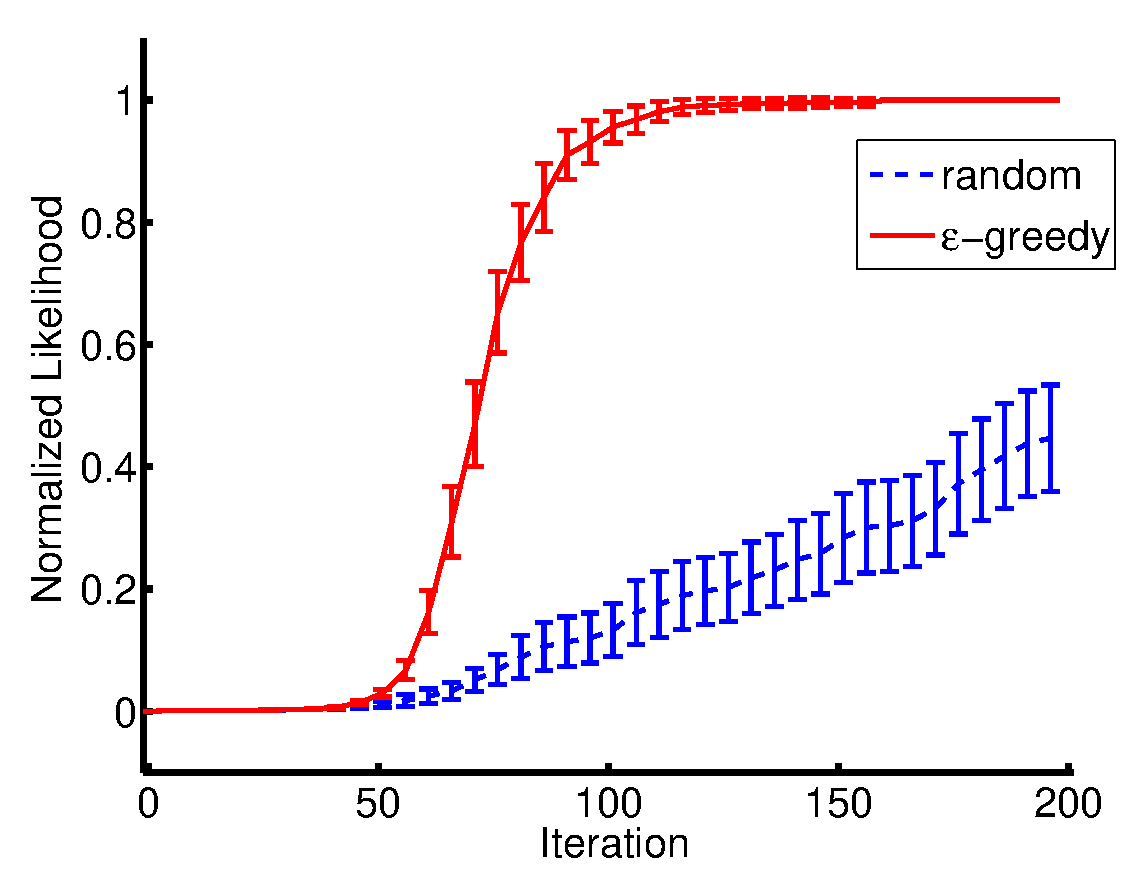
\includegraphics[width=\columnwidth]{\imgpath/feedback}
  \caption{Taught hypothesis normalized likelihood evolution (mean + standard error) thought iteration using Gaussian classifier. The teacher is providing feedback using one word per meaning. The $\epsilon$-greedy action selection method learns faster than the random one. }
  \label{fig:FeedbackGaussianRdmGreed}
\end{figure}

We will now compare the impact of using different action selection methods. From Figure~\ref{fig:FeedbackGaussianRdmGreed} we can observe that $\epsilon$-greedy results in a faster learning with less variance. This method, at each step, leads the robot in the direction of the most probable goal.
In this way it will receive more diverse feedback and will visit more relevant states than what a random exploration would do.

\subsection{Learning guidance signals}

Figure~\ref{fig:Guidance}, shows results where the teacher provides guidance instead of feedback. The number of meanings is increased from two (correct/wrong) to four (left/right/grasp/release). At each iteration the teacher first says the name of the optimal action to be performed by the robot, which then performs one action. Changes in the algorithm are described in Eq.~\ref{eq:likact}. As with feedback, the robot is able to learn the task based on guidance signals but need more iterations to reach a perfect knowledge. Indeed, even if the robot receives more informative signals, it now needs to classify instructions in four meanings which requires more samples to identify the clusters.  

\begin{figure}[!htbp]
  \centering
  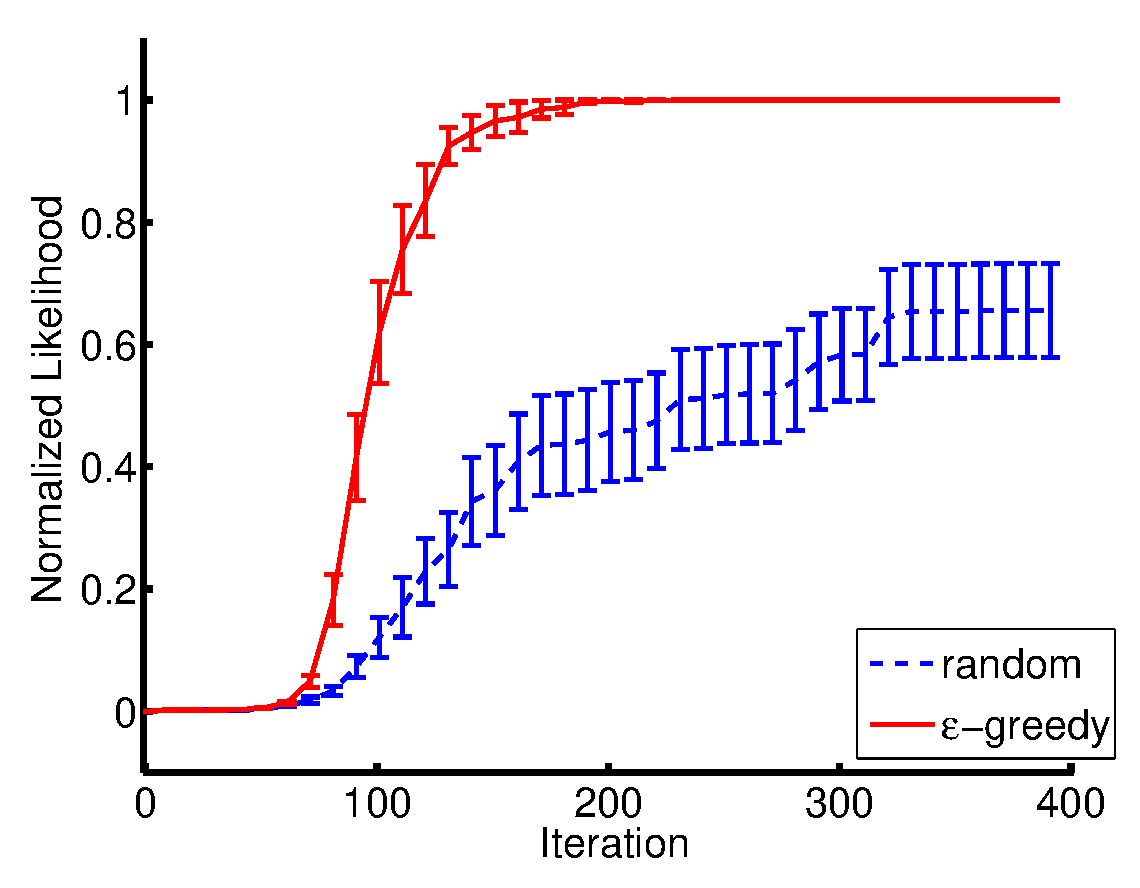
\includegraphics[width=\columnwidth]{\imgpath/guidance}
  \caption{Taught hypothesis normalized likelihood evolution (mean + standard error) thought iteration using Gaussian classifier. The teacher is providing guidance using one word per action name. The $\epsilon$-greedy action selection method learns faster than the random one. }
  \label{fig:Guidance}
\end{figure}

\subsection{Robustness to teaching mistakes}

In the results presented until now, we made the assumption that the teacher is providing feedback or guidance signals without any mistake. But real world interactions are not perfect and people can fail in providing correct feedback. An analysis of robustness is shown in figure~\ref{fig:Noise} using feedback signals, Gaussian classifier and one word per meaning. Results with and without EM are compared to study if EM is improving robustness to teaching mistakes.

\begin{figure}[!htbp]
  \centering
  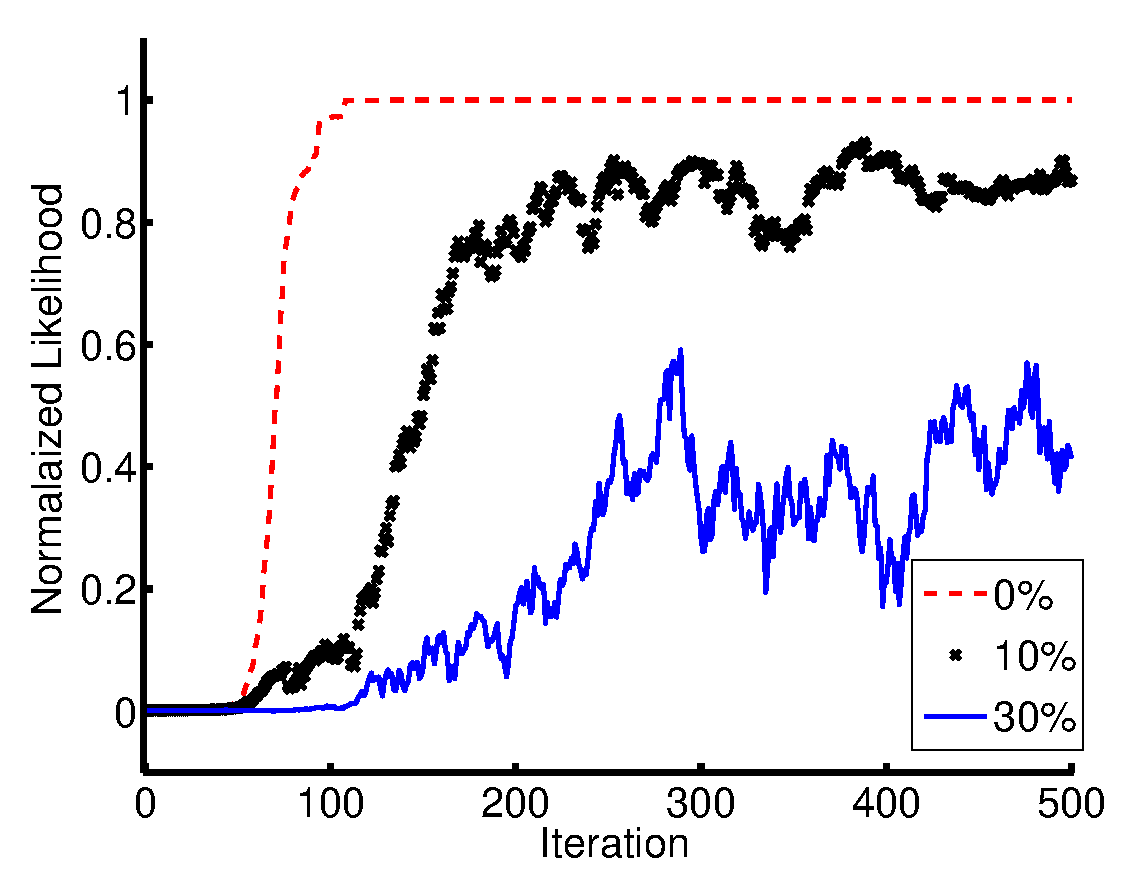
\includegraphics[width=0.49\columnwidth]{\imgpath/noise_no_EM}
  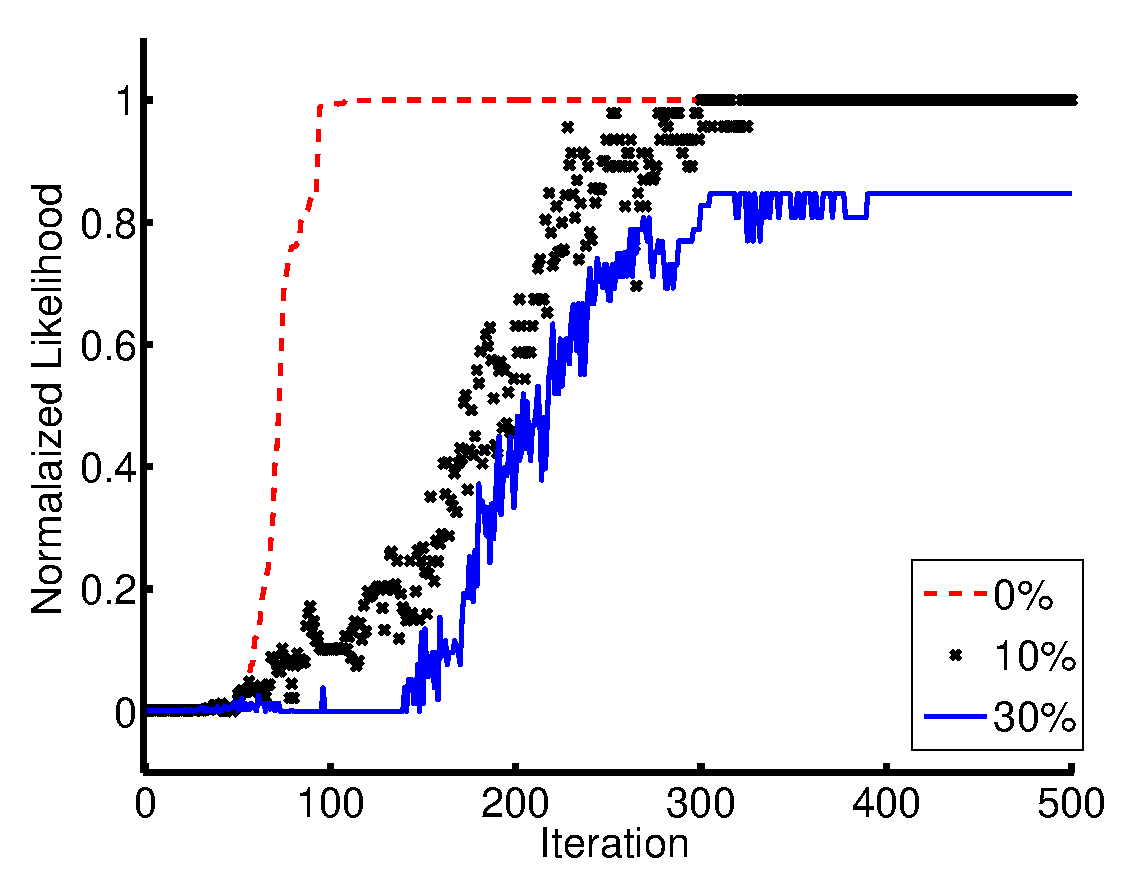
\includegraphics[width=0.49\columnwidth]{\imgpath/noise_with_EM}
  \caption{Taught hypothesis normalized likelihood evolution thought iteration using Gaussian classifier. Comparison without EM (top) versus EM (bottom). The teacher is providing feedback using one word per meaning with different percentage of mistakes. $\epsilon$-greedy action selection. Standard error has been omitted for readability reason.}
  \label{fig:Noise}
\end{figure}

We can observe that EM is performing as expected and enables the agent to identify the task more reliably facing teaching mistakes.

\subsection{Including prior information}
\label{sec:IncludingPriorInformation}

Learning purely from unknown teaching signals is challenging for the researcher but could be restrictive for the teacher. Therefore sources of known feedback could be added, such as a green and red button, where the green button has a predefined association with a \texttt{correct} feedback meaning, as red button with a \texttt{wrong} meaning. Yet, we shall expect that even in this case, users will use more modalities than the predefined one. 
%
In this study, the teacher still provides initially unknown spoken words feedback but can also use the red and green button as described in figure~\ref{bloc}. However, and in order to avoid the possibility of direct button to signal association, it can never use both modalities at the same time and use them alternatively with equal probability. 
%
Therefore, in average, after 250 iterations the robot has received 125 known feedback and 125 unknown speech signals. In most systems half of the information would be ignored but our method enable learning from the unknown signals. We study three learning methods: in the first case, the robot is learning only via the known feedback, i.e. the buttons; in the second it uses only the vocal unknown signal; and in the third one, it uses both.  Figure~\ref{fig:button} shows result from this setting. 

\begin{figure}[!htbp]
  \centering
  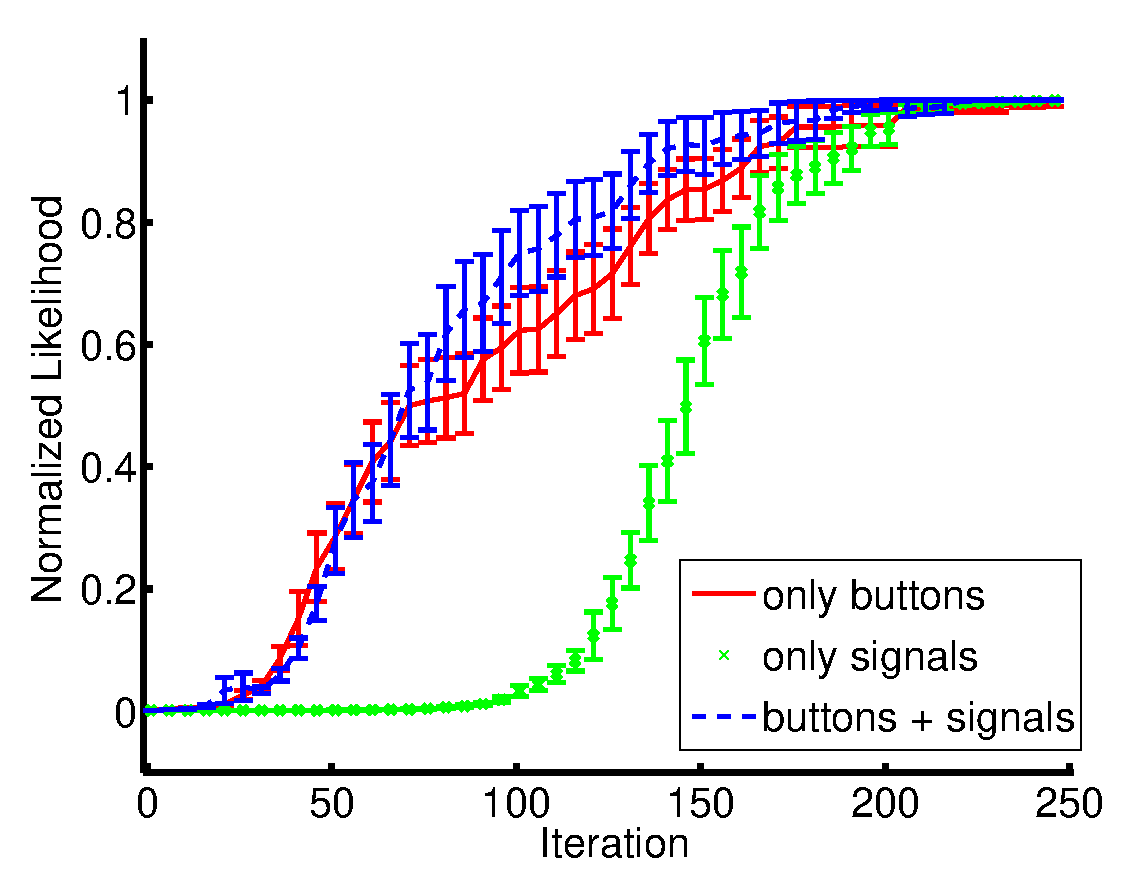
\includegraphics[width=\columnwidth]{\imgpath/mix_button}
  \caption{Taught hypothesis normalized likelihood evolution (mean + standard error) thought iteration using Gaussian classifier. Comparison of using known button, unknown signals and both.}
  \label{fig:button}
\end{figure}

As expected, learning from known feedback is faster than with unknown, however taking advantage of different sources of information, even a priori unknown, can led to slightly better performances than using only known information. Importantly, the signals to meaning knowledge of the robot is updated and could therefore be reused in further interaction.

\subsubsection{Reuse using a real robot}

Statistical simulations have shown that our algorithm allows an agent to learn a task from unknown feedback in a limited amount of interactions. To bridge the gap of simulation we tested our algorithm in real interaction condition with our robotic arm. In this experiment, the teacher is facing the robot and chooses a specific goal to reach (i.e. a specific arrangement of cubes he wants the robot to build). He then decides one word to use as positive feedback and one as negative feedback and starts to teach the robot. For this experiment the word \textit{'yes'} and \textit{'no'} were respectively used for the meaning \texttt{correct} and \texttt{wrong}. Once this  experiment is terminated we keep in memory the classifier corresponding to the best task, i.e. having the higher likelihood value, and start a new experiment where the human teacher is going to use the same feedback signals to teach a new task. But this time the spoken words are first classified as correct or wrong meaning according to the previously learnt classifier. Therefore standard IRL algorithms can be used. We study here two things, first does our system bridges the reality gap and can we reuse information learnt from a previous experience? 

\begin{figure}[!htbp]
  \centering
  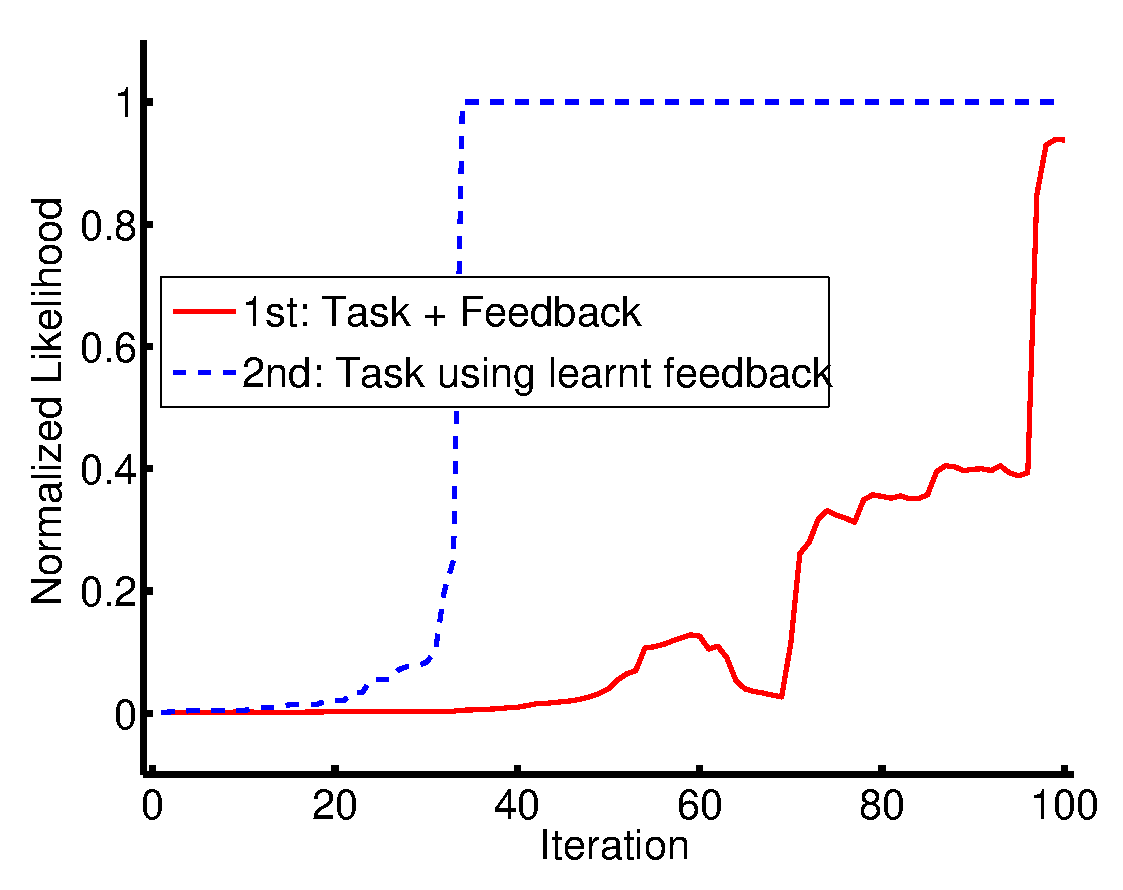
\includegraphics[width=\columnwidth]{\imgpath/real}
  \caption{Taught hypothesis normalized likelihood evolution thought iteration using Gaussian classifier.  Feedback using one word per action. $\epsilon$-greedy action selection. A first run of 100 iterations is performed where the robot learns a task from unknown feedback. Then by freezing the classifier corresponding to the best task estimate, the user teaches the robot a new task.}
  \label{Real}
\end{figure}

Figure~\ref{Real} shows results from this setting. In the first run it takes about 100 iterations for the robot to learn the task. Whereas in the second run, when reusing knowledge from the first one, the robot is able to learn a new task faster, in about 30 iterations, meaning that it has well found the two clusters in our $\mathbb{R}^{20}$ dimensional space as well as the mapping to their corresponding meaning. One of the author was the user for this studies and was aware of the task representation used by the robot, i.e. a MDP with four discrete actions. As explained in Section~\ref{sec:Introduction} an important challenge is to deal with non-expert humans whose teaching styles can vary considerably. However this challenge is not part of the current study and we note that different non-informed users teaching the robot had different understanding of the robot behaviors which led to some unsuccessful interactions (see \cite{thomaz2008teachable} for related studies).

%%%%%%%%%%%%%%%%%%%%%%%%%%%%%%%%%%%%%%%%%%%%%%
%%%%%%%%%%%%%%%%%%%%%%%%%%%%%%%%%%%%%%%%%%%%%%
%%%%%%%%%%%%%%%%%%%%%%%%%%%%%%%%%%%%%%%%%%%%%%
%%%%%%%%%%%%%%%%%%%%%%%%%%%%%%%%%%%%%%%%%%%%%%
%%%%%%%%%%%%%%%%%%%%%%%%%%%%%%%%%%%%%%%%%%%%%%
\section{Discussion}

In this work we presented an interactive learning system that can learn the initially unknown association between unlabeled instruction signals and their meaning while learning a new task. We presented empirical results showing that 1) our system can learn from unknown feedback, unknown guidance instruction signals, or a mixture of these signals, 2) it can recover from teaching mistakes, 3) it can leverage additional known sources of information, and 4) different standard classifiers can be used. An experiment with a real robot and a real user showed that 5) it can reuse acquired knowledge about human instruction signals in the learning of a new task. Finally we presented an extended experiment that mixed unknown feedback and guidance instructions, in a continuous environement, and showed that 6) an uncertainty based planning algorithm, using uncertainty from both task estimation and instruction classification, is the most efficient strategy.

\subsection{Instruction modalities} Instruction signals were here conveyed using speech sounds (which may have been interjections, or even sounds of clapping or tapping hands). Of particular interest is the possibility to use the same system with multiple modalities for instruction signals, such as facial expressions or hand gestures. This allows different users to use the system according to their own modality preferences, potentially related to their own skills and limitations. In principle, since no part of the system is specific to the sound modality, and since the sound modality is already relatively complex, there are no theoretical obstacle for this experimental extension. An interesting example might be to consider brain-computer interfaces system \cite{chavarriaga2010learning, iturrate2010robot} that usually require a long an explicit training phase. Using our system we would be able to simultaneously understand the meaning of brain signals and what task is the user trying to achieve. We started investigating in that direction with promising preliminary results \cite{grizou2013zero}.




